\documentclass[tikz]{standalone}
\usepackage{pgfplots}
\pgfplotsset{compat=1.18}
\begin{document}
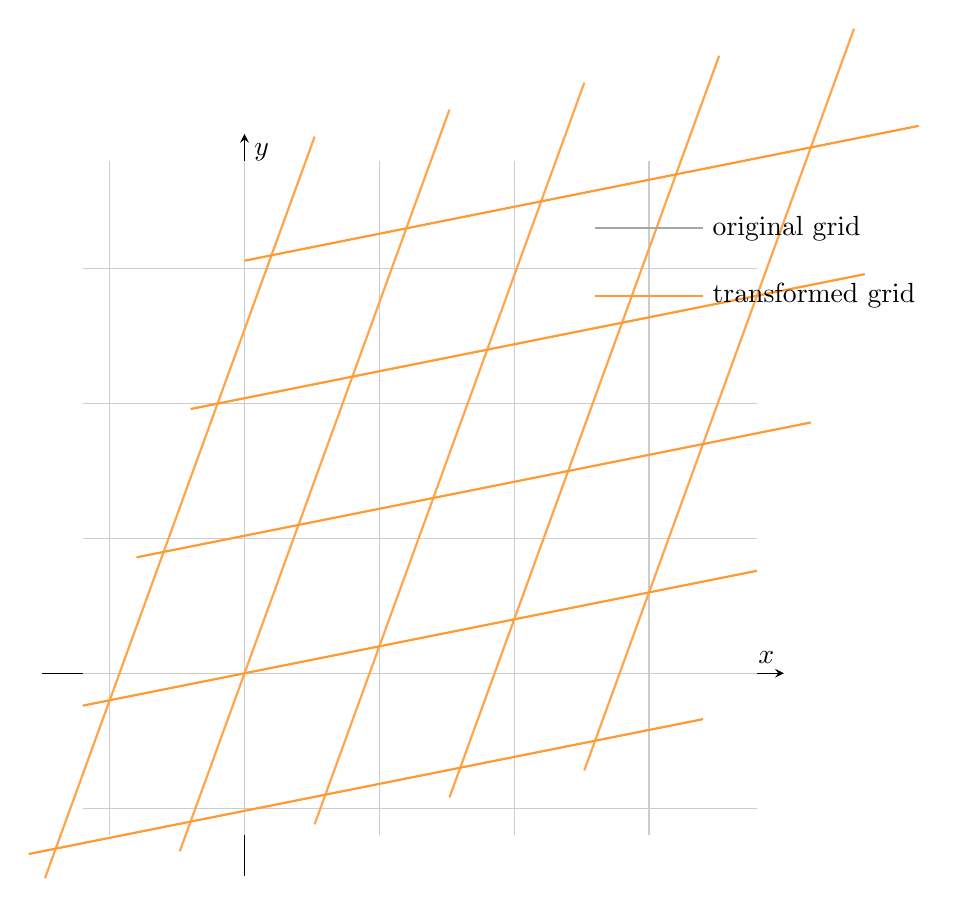
\begin{tikzpicture}
  \begin{axis}[
      axis lines=middle,
      xmin=-1.5, xmax=4,
      ymin=-1.5, ymax=4,
      xlabel={$x$}, ylabel={$y$},
      ticks=none,
      clip=false,
      width=11cm, height=11cm
  ]
    % original grid
    \foreach \x in {-1,0,1,2,3} {
      \addplot[gray!40] coordinates {(\x,-1.2) (\x,3.8)};
    }
    \foreach \y in {-1,0,1,2,3} {
      \addplot[gray!40] coordinates {(-1.2,\y) (3.8,\y)};
    }

    % transformed grid using v1=(1,0.2), v2=(0.4,1.1)
    \pgfmathsetmacro{\vOneX}{1}
    \pgfmathsetmacro{\vOneY}{0.2}
    \pgfmathsetmacro{\vTwoX}{0.4}
    \pgfmathsetmacro{\vTwoY}{1.1}
    \foreach \k in {-1,...,3} {
      \addplot[orange!70, thick] coordinates {(\k*\vOneX-1.2*\vTwoX, \k*\vOneY-1.2*\vTwoY) (\k*\vOneX+3.8*\vTwoX, \k*\vOneY+3.8*\vTwoY)};
    }
    \foreach \k in {-1,...,3} {
      \addplot[orange!80, thick] coordinates {(-1.2*\vOneX+\k*\vTwoX, -1.2*\vOneY+\k*\vTwoY) (3.8*\vOneX+\k*\vTwoX, 3.8*\vOneY+\k*\vTwoY)};
    }

    % legend markers
    \addplot[gray!70, thick] coordinates {(2.6,3.3) (3.4,3.3)};
    \node[anchor=west] at (axis cs:3.4,3.3) {original grid};
    \addplot[orange!80, thick] coordinates {(2.6,2.8) (3.4,2.8)};
    \node[anchor=west] at (axis cs:3.4,2.8) {transformed grid};
  \end{axis}
\end{tikzpicture}
\end{document}
